\documentclass[border=10pt]{standalone}

\usepackage{tikz}
\usepackage{tikzsymbols}
\usetikzlibrary{calc,patterns,shapes.geometric}

\def\centerarc[#1](#2)(#3:#4:#5){\draw[#1] ($(#2)+({#5*cos(#3)},{#5*sin(#3)})$) arc (#3:#4:#5);}

\begin{document}
	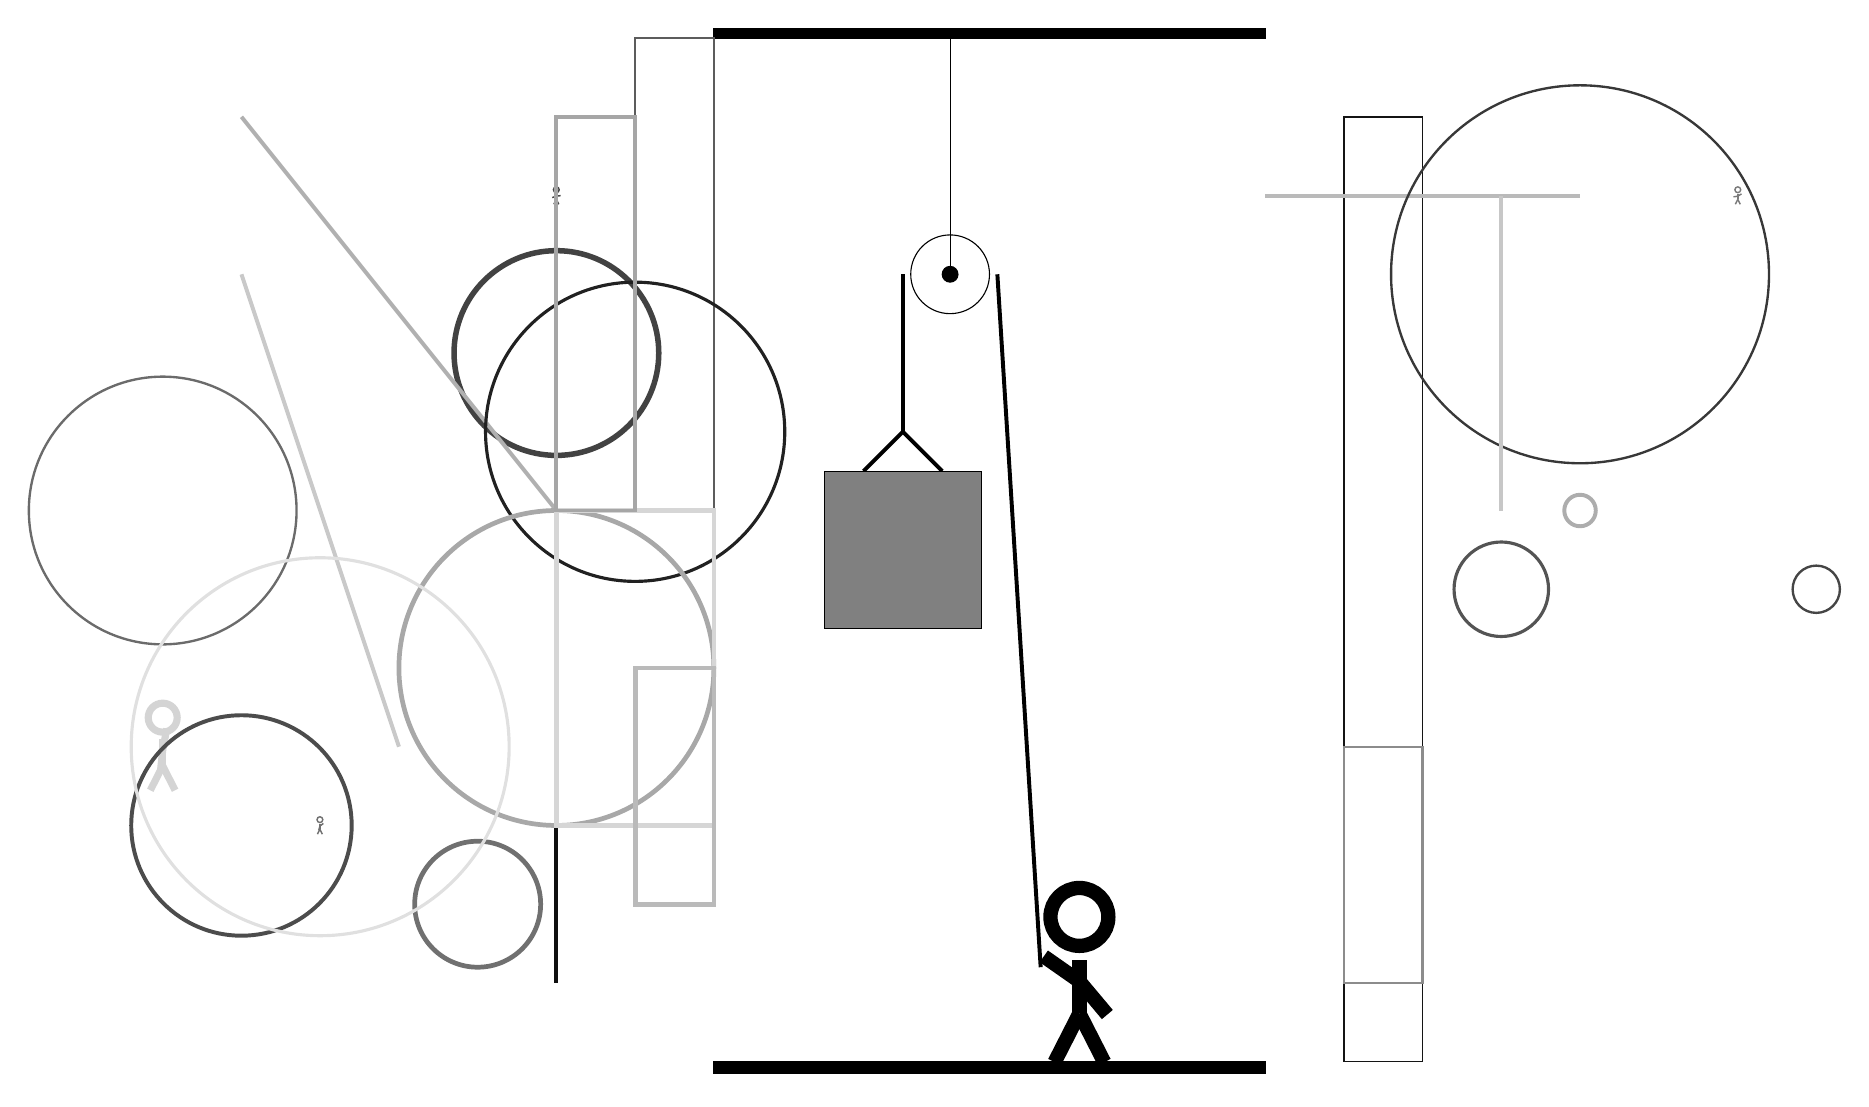
\begin{tikzpicture}
		%%%%% START %%%%%
		
		\draw[fill=black] (-2, 10) rectangle (5, 10.125);
		
		\draw (1, 7) circle (0.5);
		\draw[fill=black] (1, 7) circle (0.1);
		\draw (1, 10) -- (1, 7);
		
		\draw[line width=0.5mm] (-0.1, 4.5) -- (0.4, 5.0) -- (0.9, 4.5);
		\draw[fill=black!50] (-0.6, 4.5) rectangle (1.4, 2.5);
		
		\draw [line width=0.3mm, color=black!73](12, 3) circle (0.3);
		
		\draw [line width=0.4mm, color=black!67](8, 3) circle (0.6);
		\draw[line width=0.2mm, color=black!64] (-3, 4) rectangle (-2, 10);
		\node[line width=0.5mm, color=black!52] at (11, 8) {\Strichmaxerl[1][9][31]};
		\draw [line width=0.7mm, color=black!74](-4, 6) circle (1.3);
		
		\node[line width=0.5mm, color=black!56] at (-7, 0) {\Strichmaxerl[1][74][37]};
		
		\draw[line width=0.2mm, color=black!92] (7, -3) rectangle (6, 9);
		
		\draw [line width=0.3mm, color=black!58](-9, 4) circle (1.7);
		\draw[line width=0.5mm, color=black!21](-6, 1) -- (-8, 7);
		
		\draw[line width=0.5mm, color=black!31](-4, 4) -- (-8, 9);
		\draw[line width=0.5mm, color=black!94] (-4, -2) rectangle (-4, 1);
		\node[line width=0.4mm, color=black!72] at (-4, 8) {\Strichmaxerl[1][19][7]};
		\draw [line width=0.4mm, color=black!87](-3, 5) circle (1.9);
		
		\draw [line width=0.5mm, color=black!32](9, 4) circle (0.2);
		\draw[line width=0.5mm, color=black!27](9, 8) -- (5, 8);
		\draw [line width=0.6mm, color=black!34](-4, 2) circle (2.0);
		\draw [line width=0.3mm, color=black!78](9, 7) circle (2.4);
		\draw[line width=0.5mm, color=black!22](8, 4) -- (8, 8);
		\draw[line width=0.6mm, color=black!16] (-4, 4) rectangle (-2, 0);
		\draw [line width=0.6mm, color=black!56](-5, -1) circle (0.8);
		\draw[line width=0.5mm, color=black!35] (-4, 9) rectangle (-3, 4);
		\node[line width=0.5mm, color=black!17] at (-9, 1) {\Strichmaxerl[5][84][79]};
		
		\draw [line width=0.5mm, color=black!70](-8, 0) circle (1.4);
		\draw[line width=0.6mm, color=black!27] (-2, 2) rectangle (-3, -1);
		\draw [line width=0.4mm, color=black!12](-7, 1) circle (2.4);
		
		\draw[line width=0.3mm, color=black!45] (7, 1) rectangle (6, -2);
		
		\draw[line width=0.5mm] (0.4, 7) -- (0.4, 5.0);
		\centerarc[line width=0.5mm](1, 7)(0:180:0.6);
		\draw[line width=0.5mm](1.6, 7) -- (2.15, -1.8);
		
		\node at (2.6, -1.9) {\Strichmaxerl[10][-35][-50]};
		
		\draw[fill=black] (-2, -3) rectangle (5, -3.15);
		
		%%%%% END %%%%%
	\end{tikzpicture}
\end{document}